\documentclass[../main.tex]{subfiles}

\begin{document}

\label{cha:cha_P_14_3_3}
\subsection{Quantification of Error of Linear Regression}

\noindent Any line other than the one computed in Example 14.4 results in a larger sum of the squares of the residuals. Thus, the line is unique and in terms of our chosen criterion is a ``best'' line through the points. A number of additional properties of this fit can be elucidated by examining more closely the way in which residuals were computed. Recall that the sum of the squares is defined as [Eq. (14.12)]

\begin{equation}
	\tag{14.17}
	S_r = \sum^n_{i=1} (y_i - a_0 - a_1 x_i)^2
\end{equation}

Notice the similarity between this equation and Eq. (14.4)

\begin{equation}
\tag{14.18}
S_t = \sum (y_i - \bar{y})^2
\end{equation}
In Eq. (14.18), the square of the residual represented the square of the discrepancy between the data and a single estimate of the measure of central tendency-the mean. In Eq. (14.17), the square of the residual represents the square of the vertical distance between the data and another measure of central tendency-the straight line (\ref{fig:fig_14_9}).

\begin{wrapfigure}{l}{0.25\textwidth}
    \centering
    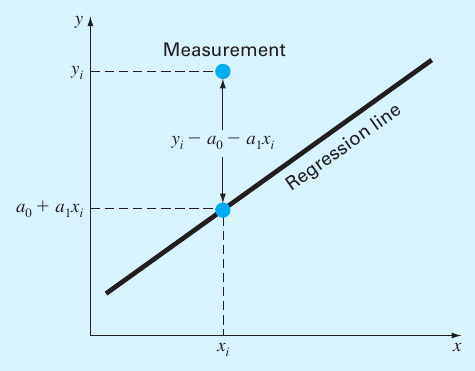
\includegraphics[width=0.25\textwidth]{fig_14_9}
   \caption{\textsf{The residual in linear regression represents the vertical distance between a data point and the straight line.}}
   \label{fig:fig_14_9}
\end{wrapfigure}

The analogy can be extended further for cases where (1) the spread of the points around the line is of similar magnitude along the entire range of the data and (2) the distribution of these points about the line is normal. It can be demonstrated that if these criteria are met, least-squares regression will provide the best (i.e., the most likely) estimates of $a_0$ and $a_1$ (Draper and Smith, 1981). This is called the maximum likelihood principle in statistics. In addition, if these criteria are met, a ``standard deviation'' for the regression line can be determined as [compare with Eq. (14.3)]

\begin{equation}
	\tag{14.19}
	s_{y/x} = \sqrt{\frac{S_r}{n-2}}
\end{equation}

\noindent where $s_{y/x}$ is called the \textit{standard error of the estimate}. The subscript notation ``$y/x$'' designates that the error is for a predicted value of $y$ corresponding to a particular value of $x$.
Also, notice that we now divide by $n - 2$ because two data-derived estimates - $a_0$ and $a_1$ — were used to compute $S_r$; thus, we have lost two degrees of freedom. As with our discussion of the standard deviation, another justification for dividing by $n - 2$ is that there is no such thing as the ``spread of data'' around a straight line connecting two points. Thus, for the case where $n = 2$, Eq. (14.19) yields a meaningless result of infinity.

Just as was the case with the standard deviation, the standard error of the estimate quantifies the spread of the data. However, $s_{y/x}$ quantifies the spread \textit{around the regression line} as shown in \ref{fig:fig_14_10b} in contrast to the standard deviation $s_y$ that quantified the \textit{spread around the mean} (\ref{fig:fig_14_10a}).

\begin{figure}[H]
	\centering
	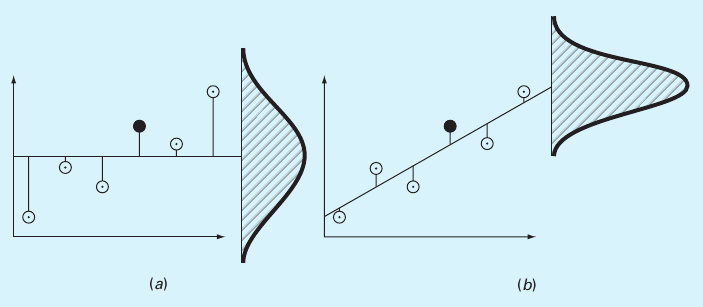
\includegraphics[width=1\linewidth]{fig_14_10}
	\caption{\textsf{Regression data showing (a) the spread of the data around the mean of the dependent variable and (b) the spread of the data around the best-fit line. The reduction in the spread in going from (a) to (b), as indicated by the bell-shaped curves at the right, represents the improvement due to linear regression.}}
	\label{fig:fig_14_10}
	\label{fig:fig_14_10a}
	\label{fig:fig_14_10b}
\end{figure}

\begin{figure}[H]
	\centering
	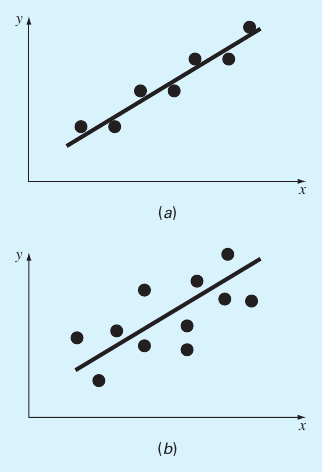
\includegraphics[width=1\linewidth]{fig_14_11}
	\caption{\textsf{Examples of linear regression with (a) small and (b) large residual errors.}}
	\label{fig:fig_14_11}
	\label{fig:fig_14_11a}
	\label{fig:fig_14_11b}
\end{figure}

These concepts can be used to quantify the ``goodness'' of our fit. This is particularly useful for comparison of several regressions (\ref{fig:fig_14_11a}). To do this, we return to the original data and determine the total sum of the squares around the mean for the dependent variable (in our case, $y$). As was the case for Eq. (14.18), this quantity is designated $S_t$. This is the magnitude of the residual error associated with the dependent variable prior to regression. After performing the regression, we can compute $S_r$, the sum of the squares of the residuals around the regression line with Eq. (14.17). This characterizes the residual error that remains after the regression. It is, therefore, sometimes called the unexplained sum of the squares. The difference between the two quantities, $S_t - S_r$, quantifies the improvement or error reduction due to describing the data in terms of a straight line rather than as an average value. Because the magnitude of this quantity is scale-dependent, the difference is normalized to $S_t$ to yield

\begin{equation}
	\tag{14.20}
	r^2 = \frac{S_t - S_r}{S_t}
\end{equation}

\noindent where $r^2$ is called the \textit{coefficient of determination} and $r$ is the \textit{correlation coefficient} ($=\sqrt{r^2}$). For a perfect fit, $S_r = 0$ and $r^2 = 1$, signifying that the line explains 100\% of the variability of the data. For $r^2 = 0$, $S_r = S_t$ and the fit represents no improvement. An alternative formulation for $r$ that is more convenient for computer implementation is

\begin{equation}
	\tag{14.21}
	r = \frac{n \sum (x_i y_i) - (\sum x_i) (\sum y_i)}{\sqrt{n \sum x^2_i - (\sum x_i)^2} \sqrt{n \sum y^2_i - (\sum y_i)^2}}
\end{equation}

%TODO EXAMPLE 342

Before proceeding, a word of caution is in order. Although the coefficient of determination provides a handy measure of goodness-of-fit, you should be careful not to ascribe more meaning to it than is warranted. Just because $r^2$ is ``close'' to 1 does not mean that the fit is necessarily ``good''. For example, it is possible to obtain a relatively high value of $r^2$ when the underlying relationship between $y$ and $x$ is not even linear. Draper and Smith (1981) provide guidance and additional material regarding assessment of results for linear regression. In addition, at the minimum, you should always inspect a plot of the data along with your regression curve.

A nice example was developed by Anscombe (1973). As in Fig. 14.12, he came up with four data sets consisting of 11 data points each. Although their graphs are very different, all have the same best-fit equation, $y = 3 + 0.5 x$, and the same coefficient of determination, $r^2 = 0.67$! This example dramatically illustrates why developing plots is so valuable.

\begin{figure}[H]
	\centering
	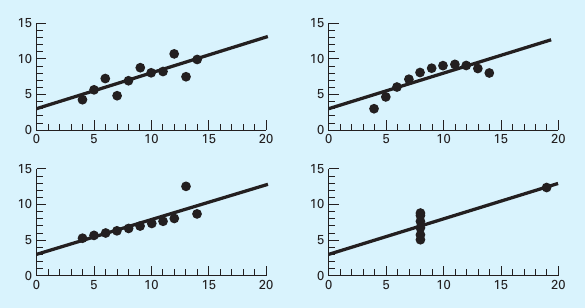
\includegraphics[width=1\linewidth]{fig_14_12}
	\caption{\textsf{Anscombe’s four data sets along with the best-fit line, $y = 3 + 0.5x$.}}
	\label{fig:fig_14_12}
\end{figure}


\label{cha:cha_P_14_4}
\section{LINEARIZATION OF NONLINEAR RELATIONSHIPS}

Linear regression provides a powerful technique for fitting a best line to data. However, it is predicated on the fact that the relationship between the dependent and independent variables is linear. This is not always the case, and the first step in any regression analysis should be to plot and visually inspect the data to ascertain whether a linear model applies. In some cases, techniques such as polynomial regression, which is described in Chap. 15, are appropriate. For others, transformations can be used to express the data in a form that is compatible with linear regression.

One example is the \textit{exponential model}:

\begin{equation}
	\tag{14.22}
	y = a_1 e^{\beta_1 x}
\end{equation}

\noindent where $\alpha$ and $\beta_1$ are constants. This model is used in many fields of engineering and science to characterize quantities that increase (positive $\beta_1$) or decrease (negative $\beta_1$) at a rate that is directly proportional to their own magnitude. For example, population growth or radioactive decay can exhibit such behavior. As depicted in Fig. 14.13a, the equation represents a nonlinear relationship (for $\beta_1 \neq 0$) between $y$ and $x$.

Another example of a nonlinear model is the simple \textit{power equation:}

\begin{equation}
\tag{14.23}
y = a_2 x^{\beta_2}
\end{equation}

\noindent where $\alpha_2$ and $\beta_2$ are constant coefficients. This model has wide applicability in all fields of engineering and science. It is very frequently used to fit experimental data when the underlying model is not known. As depicted in Fig. 14.13b, the equation (for $\beta_2 \neq 0$) is nonlinear.

\begin{figure}[H]
	\centering
	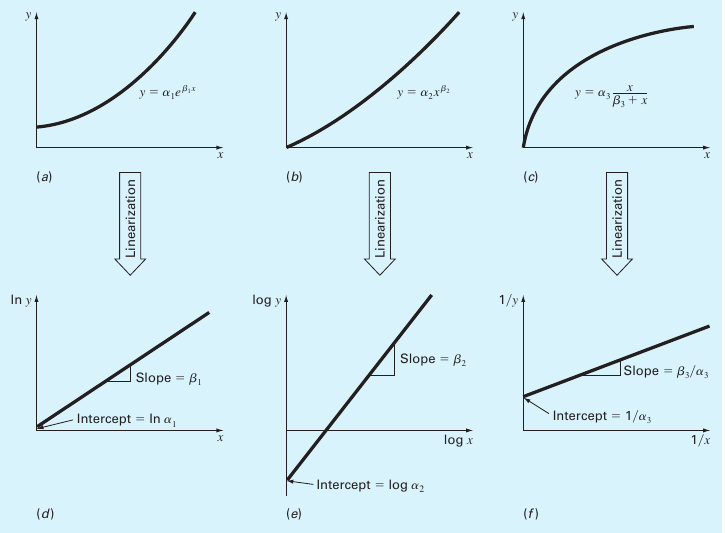
\includegraphics[width=1\linewidth]{fig_14_13}
	\caption{\textsf{(a) The exponential equation, (b) the power equation, and (c) the saturation-growth-rate equation. Parts (d), (e), and (f) are linearized versions of these equations that result from simple transformations.}}
	\label{fig:fig_14_13}
	\label{fig:fig_14_13a}
	\label{fig:fig_14_13b}
	\label{fig:fig_14_13c}
	\label{fig:fig_14_13d}
	\label{fig:fig_14_13e}
	\label{fig:fig_14_13f}
\end{figure}


A third example of a nonlinear model is the \textit{saturation-growth-rate equation}:

\begin{equation}
	\tag{14.24}
	y = \alpha_3 \frac{x}{\beta_3 + x}
\end{equation}

\noindent where $\alpha_3$ and $\beta_3$ are constant coefficients. This model, which is particularly well-suited for characterizing population growth rate under limiting conditions, also represents a nonlinear relationship between y and x (Fig. 14.13c) that levels off, or “saturates,” as $x$ increases. It has many applications, particularly in biologically related areas of both engineering and science.

Nonlinear regression techniques are available to fit these equations to experimental data directly. However, a simpler alternative is to use mathematical manipulations to trans form the equations into a linear form. Then linear regression can be employed to fit the equations to data.

For example, Eq. (14.22) can be linearized by taking its natural logarithm to yield

\begin{equation}
	\tag{14.25}
	\ln{y} = \ln{\alpha_1} + \beta_1 x
\end{equation}

\noindent Thus, a plot of $\ln{y}$ versus $x$ will yield a straight line with a slope of $\beta_1$ and an intercept of $\ln{\alpha_1}$ (Fig. 14.13d).

Equation (14.23) is linearized by taking its base-10 logarithm to give

\begin{equation} % Page 346
	\tag{14.26}
	\log y = \log \alpha_2 + \beta_2 \log x
\end{equation} 

\noindent Thus, a plot of log y versus log x will yield a straight line with a slope of $\beta_2$ and an intercept of $\log \alpha_2$ (Fig. 14.13e). Note that any base logarithm can be used to linearize this model. However, as done here, the base-10 logarithm is most commonly employed.

Equation (14.24) is linearized by inverting it to give

\begin{equation}
	\tag{14.27}
	\frac{1}{y} = \frac{1}{\alpha_3} + \frac{\beta_3}{\alpha_3} \frac{1}{x}
\end{equation}

\noindent Thus, a plot of $1/y$ versus $1/x$ will be linear, with a slope of $\beta_3 / \alpha_3$ and an intercept of $1 / \alpha_3$ (Fig. 14.13f).

In their transformed forms, these models can be fit with linear regression to evaluate the constant coefficients. They can then be transformed back to their original state and used for predictive purposes. The following illustrates this procedure for the power model.

% TODO EXAMPLE 14.6 346


The fits in Example 14.6 (Fig. 14.14) should be compared with the one obtained previously in Example 14.4 (Fig. 14.8) using linear regression on the untransformed data. Although both results would appear to be acceptable, the transformed result has the advantage that it does not yield negative force predictions at low velocities. Further, it is known from the discipline of fluid mechanics that the drag force on an object moving through a fluid is often well described by a model with velocity squared. Thus, knowledge from the field you are studying often has a large bearing on the choice of the appropriate model equation you use for curve fitting.


\label{cha:cha_P_14_4_1}
\subsection{General Comments on Linear Regression}

\noindent Before proceeding to curvilinear and multiple linear regression, we must emphasize the introductory nature of the foregoing material on linear regression. We have focused on the simple derivation and practical use of equations to fit data. You should be cognizant of the fact that there are theoretical aspects of regression that are of practical importance but are beyond the scope of this book. For example, some statistical assumptions that are inherent in the linear least-squares procedures are

\begin{enumerate}
	\item Each $x$ has a fixed value; it is not random and is known without error.
	\item The $y$ values are independent random variables and all have the same variance.
	\item The $y$ values for a given $x$ must be normally distributed.
\end{enumerate}

Such assumptions are relevant to the proper derivation and use of regression. For example, the first assumption means that (1) the $x$ values must be error-free and (2) the regression of $y$ versus $x$ is not the same as $x$ versus $y$. You are urged to consult other references such as Draper and Smith (1981) to appreciate aspects and nuances of regression that are beyond the scope of this book.

\label{cha:cha_P_14_5}
\section{COMPUTER APPLICATIONS}

\noindent Linear regression is so commonplace that it can be implemented on most pocket calculators. In this section, we will show how a simple M-file can be developed to determine the slope and intercept as well as to create a plot of the data and the best-fit line. We will also show how linear regression can be implemented with the built-in \texttt{polyfit} function.

\label{cha:cha_P_14_5_1}
\subsection{MATLAB M-file: \texttt{linregr}}
\noindent An algorithm for linear regression can be easily developed (Fig. 14.15). The required summations are readily computed with MATLAB's \texttt{sum} function. These are then used to compute the slope and the intercept with Eqs. (14.15) and (14.16). The routine displays the intercept and slope, the coefficient of determination, and a plot of the best-fit line along with the measurements.


A simple example of the use of this M-file would be to fit the force-velocity data analyzed in Example 14.4:

%TODO EXAMPLE 14.1 349


\label{cha:cha_P_14_5_2} %351
\subsection{MATLAB Functions: \texttt{polyfit} and \texttt{polyval}}

\noindent MATLAB has a built-in function \texttt{polyfit} that fits a least-squares \textit{n}th-order polynomial to data. It can be applied as in

\begin{lstlisting}[numbers=none]
>> p = polyfit(x, y, n)
\end{lstlisting}

\noindent where $x$ and $y$ are the vectors of the independent and the dependent variabless, respectively, and $n =$ the order of the polynomial. The function returns a vector $p$ containing the polynomial's coefficients. We should note that it represents the polynomial using decreasing powers of $x$ as in the following representation:

\begin{equation}
	f(x) = p_1x^n + p_2x^{n-1} + \cdots + p_n x + p_{n + 1}
\end{equation}

Because a straight line is a first-order polynomial, \verb|polyfit(x,y,1)| will return the slope and the intercept of the best-fit straight line.

\begin{lstlisting}[numbers=none]
>> x = [10 20 30 40 50 60 70 80];
>> y = [25 70 380 550 610 1220 830 1450];
>> a = polyfit(x,y,1)
a =
	19.4702 -234.2857
\end{lstlisting}

\noindent Thus, the slope is 19.4702 and the intercept is -234.2857.

Another function, \texttt{polyval}, can then be used to compute a value using the coefficients. It has the general format:

\begin{lstlisting}[numbers=none]
>> y = polyval(p, x)
\end{lstlisting}

\noindent where $p =$ the polynomial coefficients, and $y =$ the best-fit value at $x$. For example,

\begin{lstlisting}[numbers=none]
>> y = polyval(a,45)
y =
	641.8750
\end{lstlisting}

\bigskip

% ENZYME KINETICS
\textbf{Background.} \textit{Enzymes} act as catalysts to speed up the rate of chemical reactions in living cells. In most cases, they convert one chemical, the \textit{substrate},into another, the \textit{product}. The \textit{Michaelis-Menten} equation is commonly used to describe such reactions:

\begin{equation}
	v = \frac{v_m[S]}{k_s + [S]}
\end{equation}

\noindent where $v =$ the initial reaction velocity, $v_m =$ the maximum initial reaction velocity, $[S] =$ substrate concentration, and $k_s =$ a half-saturation constant. As in Fig. 14.16, the equation describes a saturating relationship which levels off with increasing $[S]$. The graph also illustrates that the \textit{half-saturation constant} corresponds to the substrate concentration at which the velocity is half the maximum.

\begin{figure}[H] % Page 352
	\centering
	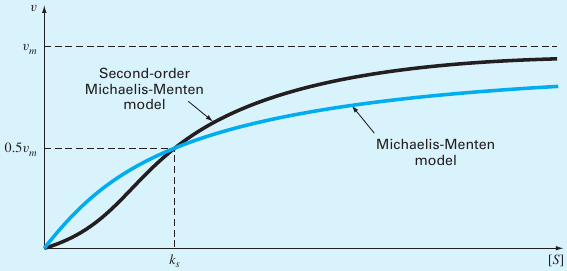
\includegraphics[width=1\linewidth]{fig_14_16}
	\caption{\textsf{Two versions of the Michaelis-Menten model of enzyme kinetics.}}
	\label{fig:fig_14_16}
\end{figure}

Although the Michaelis-Menten model provides a nice starting point, it has been refined and extended to incorporate additional features of enzyme kinetics. One simple extension involves so-called \textit{allosteric enzymes}, where the binding of a substrate molecule at one site leads to enhanced binding of subsequent molecules at other sites. For cases with two interacting bonding sites, the following second-order version often results in a better fit:

\begin{equation}
	v = \frac{v_m {[S]}^2}{k^2_s + {[S]}^2}
\end{equation}

\noindent This model also describes a saturating curve but, as depicted in Fig. 14.16, the squared concentrations tend to make the shape more \textit{sigmoid},or S-shaped.

Suppose that you are provided with the following data:
% todo this should be a table
\begin{lstlisting}[numbers=none] 
[S] 1.3  1.8  3    4.5   6     8    9
v   0.07 0.13 0.22 0.275 0.335 0.35 0.36
\end{lstlisting}

\noindent Employ linear regression to fit these data with linearized versions of Eqs. (14.28) and (14.29). Aside from estimating the model parameters, assess the validity of the fits with both statistical measures and graphs.

\textbf{Solution.} Equation (14.28), which is in the format of the saturation-growth-rate model (Eq. 14.24), can be linearized by inverting it to give (recall Eq. 14.27)

\begin{equation}
	\frac{1}{v} = \frac{1}{v_m} + \frac{k_s}{v_m} \frac{1}{[S]}
\end{equation}

\noindent The \texttt{linregr} function from Fig. 14.15 can then be used to determine the least-squares fit:

\begin{lstlisting}[numbers=none] 
>> S=[1.3 1.8 3 4.5 6 8 9];
>> v=[0.07 0.13 0.22 0.275 0.335 0.35 0.36];
>> [a,r2]=linregr(1./S,1./v)
a =
16.4022
 0.1902
r2 =
0.9344
\end{lstlisting}

\noindent The model coefficients can then be calculated as

\begin{lstlisting}[numbers=none] 
>> vm=1/a(2)
vm =
5.2570
>> ks=vm*a(1)
ks =
86.2260
\end{lstlisting}

\noindent Thus, the best-fit model is

\begin{equation}
	v = \frac{5.2570[S]}{86.2260 + [S]}
\end{equation}

Although the high value of $r^2$ might lead you to believe that this result is acceptable, inspection of the coefficients might raise doubts. For example, the maximum velocity (5.2570) is much greater than the highest observed velocity (0.36). In addition, the half-saturation rate (86.2260) is much bigger than the maximum substrate concentration (9).

The problem is underscored when the fit is plotted along with the data. Figure 14.17a shows the transformed version. Although the straight line follows the upward trend, the data clearly appear to be curved. When the original equation is plotted along with the data in the untransformed version (Fig. 14.17b), the fit is obviously unacceptable. The data are clearly leveling off at about 0.36 or 0.37. If this is correct, an eyeball estimate would suggest that $v_m$ should be about 0.36, and $k_s$ should be in the range of 2 to 3.

Beyond the visual evidence, the poorness of the fit is also reflected by statistics like the coefficient of determination. For the untransformed case, a much less acceptable result of $r^2 = 0.6406$ is obtained.


The foregoing analysis can be repeated for the second-order model. Equation (14.28) can also be linearized by inverting it to give

\begin{equation}
	\frac{1}{v} = \frac{1}{v_m} + \frac{k^2_s}{v_m} \frac{1}{[S]^2}
\end{equation}

The \texttt{linregr} function from Fig. 14.15 can again be used to determine the least-squares fit:

\begin{lstlisting}[numbers=none] 
>> [a,r2]=linregr(1./S.^2,1./v)
a =
19.3760
 2.4492
r2 =
0.9929
\end{lstlisting}

% Page 354
\begin{figure}[H] 
	\centering
	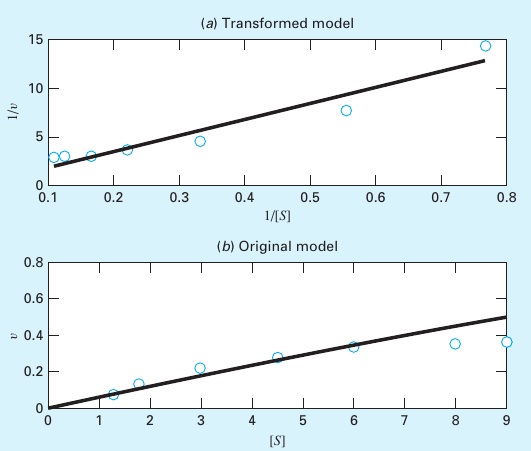
\includegraphics[width=1\linewidth]{fig_14_17}
	\caption{\textsf{Plots of least-squares fit (line) of the Michaelis-Menten model along with data (points). The plot in (a) shows the transformed fit, and (b) shows how the fit looks when viewed in the untransformed, original form.}}
	\label{fig:fig_14_17}
\end{figure}

\noindent The model coefficients can then be calculated as

\begin{lstlisting}[numbers=none] 
>> vm=1/a(2)
vm =
0.4083
>> ks=sqrt(vm*a(1))
ks =
2.8127
\end{lstlisting}

\noindent Substituting these values into Eq. (14.29) gives

\begin{equation}
	v = \frac{0.4083[S]^2}{7.911 + [S]^2}
\end{equation}

Although we know that a high $r^2$ does not guarantee of a good fit, the fact that it is very high (0.9929) is promising. In addition, the parameters values also seem consistent with the trends in the data; that is, the $k_m$ is slightly greater than the highest observed velocity and the half-saturation rate is lower than the maximum substrate concentration (9).

\begin{figure}[H] 
	\centering
	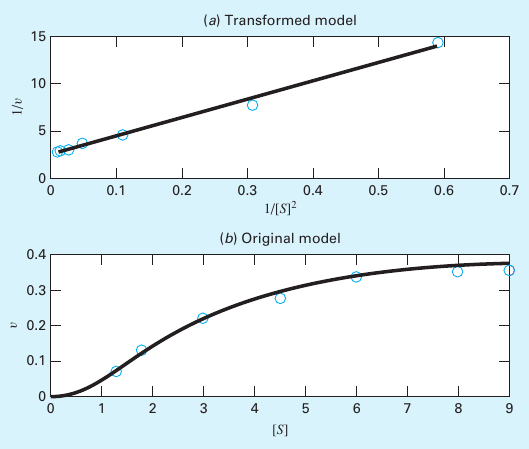
\includegraphics[width=1\linewidth]{fig_14_18}
	\caption{\textsf{Plots of least-squares fit (line) of the second-order Michaelis-Menten model along with data (points). The plot in (a) shows the transformed fit, and (b) shows the untransformed, original form.}}
	\label{fig:fig_14_18}
\end{figure}

The adequacy of the fit can be assessed graphically. As in Fig. 14.18a, the transformed results appear linear. When the original equation is plotted along with the data in the untransformed version (Fig. 14.18b), the fit nicely follows the trend in the measurements. Beyond the graphs, the goodness of the fit is also reflected by the fact that the coefficient of determination for the untransformed case can be computed as $r^2 = 0.9896$.

Based on our analysis, we can conclude that the second-order model provides a good fit of this data set. This might suggest that we are dealing with an allosteric enzyme. 

Beyond this specific result, there are a few other general conclusions that can be drawn from this case study. First, we should never solely rely on statistics such as $r^2$ as the sole basis of assessing goodness of fit. Second, regression equations should always be assessed graphically. And for cases where transformations are employed, a graph of the untransformed model and data should always be inspected. 

Finally, although transformations may yield a decent fit of the transformed data, this does not always translate into an acceptable fit in the original format. The reason that this might occur is that minimizing squared residuals of transformed data is not the same as for the untransformed data. Linear regression assumes that the scatter of points around the best-fit line follows a Gaussian distribution,  and that the standard deviation is the same at every value of the dependent variable. These assumptions are rarely true after transforming data. 

As a consequence of the last conclusion, some analysts suggest that rather than using linear transformations, nonlinear regression should be employed to fit curvilinear data. In this approach, a best-fit curve is developed that directly minimizes the untransformed residuals. We will describe how this is done in Chap. 15. %TODO chapter label
% 356

% TODO PROBLEMS

\label{cha:cha_P_15} %351
\chapter{General Linear Least-Squares and Nonlinear Regression}
\textbf{CHAPTER OBJECTIVES}

\noindent This chapter takes the concept of fitting a straight line and extends it to (a) fitting a polynomial and (b) fitting a variable that is a linear function of two or more independent variables. We will then show how such applications can be generalized and applied to a broader group of problems. Finally, we will illustrate how optimization techniques can be used to implement nonlinear regression. Specific objectives and topics covered are

\begin{list}{•}{}
	\item Knowing how to implement polynomial regression.
	\item Knowing how to implement multiple linear regression. %why FIXME
	\item Understanding the formulation of the general linear least-squares model.
	\item Understanding how the general linear least-squares model can be solved with MATLAB using either the normal equations or left division.
	\item Understanding how to implement nonlinear regression with optimization techniques.
\end{list}


\label{cha:cha_P_15_1}
\section{POLYNOMIAL REGRESSION}
\noindent In Chap.14, a procedure was developed to derive the equation of a straight line using the least-squares criterion. Some data, although exhibiting a marked pattern such as seen in Fig. 15.1, are poorly represented by a straight line. For these cases, a curve would be better suited to fit the data. As discussed in Chap. 14, one method to accomplish this objective is to use transformations. Another alternative is to fit polynomials to the data using \emph{polynomial regression}.

The least-squares procedure can be readily extended to fit the data to a higher-orderpolynomial. For example,  suppose that we fit a second-order polynomial or quadratic:

\begin{equation}
	\tag{15.1}
	y = a_0 + a_1x + a_2x^2 + e
\end{equation}

\begin{wrapfigure}{l}{0.25\textwidth}
    \centering
    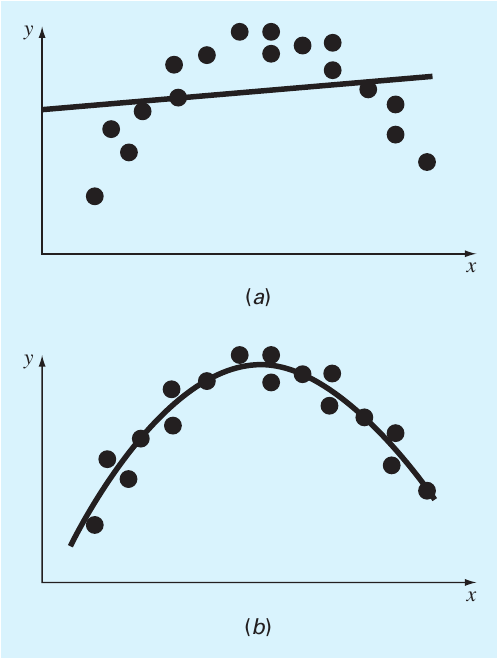
\includegraphics[width=0.25\textwidth]{fig_15_1}
   \caption{\textsf{a) Data that are ill-suited for linear least-squares regression. (b) Indication that a parabola is preferable.}}
   \label{fig:fig_15_1}
\end{wrapfigure}

\noindent For this case the sum of the squares of the residuals is

\begin{equation}
	\tag{15.2}
	S_r = \sum^n_{i=1}(y_i - a_0 - a_1x_i - a_2x^2_i)^2
\end{equation}

To generate the least-squares fit, we take the derivative of Eq. (15.2) with respect to each of the unknown coefficients of the polynomial, as in

\begin{equation}
	\frac{\partial S_r}{\partial a_0} = -2 \sum (y_i -a_0 -a_1x_i - a_2x_i^2)
\end{equation}

\begin{equation}
	\frac{\partial S_r}{\partial a_1} = -2 \sum x_i (y_i -a_0 -a_1x_i - a_2x_i^2)
\end{equation}

\begin{equation}
	\frac{\partial S_r}{\partial a_2} = -2 \sum x_i^2 (y_i -a_0 -a_1x_i - a_2x_i^2)
\end{equation}

\noindent These equations can be set equal to zero and rearranged to develop the following set of normal equations:

\begin{equation}
	(n)a_0 + (\sum x_i) a_1 + (\sum x^2_i) a_2 = \sum y_i
\end{equation}

\begin{equation}
	(\sum x_i)a_0 + (\sum x_i ^ 2) a_1 + (\sum x^3_i) a_2 = \sum x_i y_i
\end{equation}

\begin{equation}
	(\sum x_i^2)a_0 + (\sum x_i ^ 3) a_1 + (\sum x^4_i) a_2 = \sum x_i^2 y_i
\end{equation}

\noindent where all summations are from $i = 1$ through $n$. Note that the preceding three equations are linear and have three unknowns: $a_0$ , $a_1$, and $a_2$. The coefficients of the unknowns can be calculated directly from the observed data.

For this case, we see that the problem of determining a least-squares second-order polynomial is equivalent to solving a system of three simultaneous linear equations. The two-dimensional case can be easily extended to an $m$th-order polynomial as in

\begin{equation}
	y = a_0 + a_1 x + a_2 x^2 + \cdots + a_m x^m + e
\end{equation}

The foregoing analysis can be easily extended to this more general case. Thus, we can recognize that determining the coefficients of an $m$th-order polynomial is equivalent to solving a system of $m + 1$ simultaneous linear equations. For this case, the standard error is formulated as

\begin{equation}
	\tag{15.3}
	s_{y/x} = \sqrt{\frac{S_r}{n - (m + 1)}}
\end{equation}

This quantity is divided by $n - (m + 1)$ because $(m + 1)$ data-derived coefficients - $a_0, a_1, ..., a_m$ - were used to compute $S_r$; thus, we have lost $m + 1$ degrees of freedom. In addition to the standard error, a coefficient of determination can also be computed for polynomial regression with Eq. (14.20).

% TODO EXAMPLE 15.1

\label{cha:cha_P_15_2} % 365
\section{MULTIPLE LINEAR REGRESSION}

\noindent Another useful extension of linear regression is the case where $y$ is a linear function of two or more independent variables. For example, $y$ might be a linear function of $x_1$ and $x_2$, as in

\begin{equation}
	y = a_0 + a_1x_1 + a_2x_2+e
\end{equation}

\noindent Such an equation is particularly useful when fitting experimental data where the variable being studied is often a function of two other variables. For this two-dimensional case, the regression ``line'' becomes a ``plane'' (Fig. 15.3).

As with the previous cases, the "best" values of the coefficients are determined by formulating the sum of the squares of the residuals:

\begin{equation}
	\tag{15.4}
	S_r = \sum_{i=1}^n (y_i - a_0 - a_1x_{1,i} - a_2x_{2,i})^2
\end{equation}

\noindent and differentiating with respect to each of the unknown coefficients:

\begin{equation}
	\frac{\partial S_r}{\partial a_0} = -2 \sum (y_i -a_0 -a_1x_{1,i} - a_2x_{2,i}^2)
\end{equation}

\begin{equation}
	\frac{\partial S_r}{\partial a_1} = -2 \sum x_{1,i} (y_i -a_0 -a_1x_{1,i} - a_2x_{2,i}^2)
\end{equation}

\begin{equation}
	\frac{\partial S_r}{\partial a_2} = -2 \sum x_{2,i}^2 (y_i -a_0 -a_1x_{1,i} - a_2x_{2,i}^2)
\end{equation}

\begin{wrapfigure}{l}{0.25\textwidth}
    \centering
    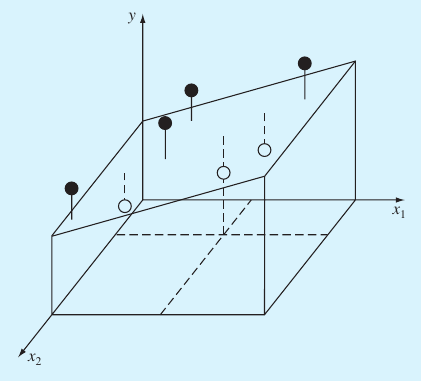
\includegraphics[width=0.25\textwidth]{fig_15_3}
   \caption{\textsf{Graphical depiction of multiple linear regression where y is a linear function of $x_1$ and $x_2$.}}
   \label{fig:fig_15_3}
\end{wrapfigure}

\noindent The coefficients yielding the minimum sum of the squares of the residuals are obtained by setting the partial derivatives equal to zero and expressing the result in matrix form as 

\begin{equation} % 366
...
\end{equation}

\end{document}
% TODO figure references, examples